

\label{sec:mechanicalDomain}
In dieser Domäne wurde exemplarisch eine partikelbasierte Fluid-Simulation nach dem
Verfahren der Smoothed Particle Hydrodynamics mit OpenCL implementiert.
	
\subsubsection{Fluid-Simulation}
		
	\paragraph{Grundlagen}
		
		\subparagraph{Die Navier-Stokes-Gleichungen}
		Die Sammlung an Gleichungen, die das Verhalten von Fluiden beschreiben, sind die
		\emph{Navier-Stokes-Gleichungen}.
		Für die Echtzeit-Simulation nützlich sind die \emph{inkompressiblen} Navier-Stokes-Gleichungen:
		\begin{subequations}\label{equ:navStokes1}
			\begin{align}
			\rho 
			\left( 
				\frac{\partial \vec{v}}{\partial t} 
				+ 
				\left( \vec{v} \cdot \nabla	\right) \vec{v} 
			\right)
				& = - \nabla p  + \mu \Delta \vec{v} + \vec{f} \\
			\nabla \cdot \vec{v}   & = 0
			\end{align}	
		\end{subequations}
		
		Die erste Gleichung heißt \emph{Impulsgleichung}. Die basiert auf dem zweiten Newtonschen Gesetz
		\begin{equation}
			\vec{F} = m \cdot \vec{a}
		\end{equation}
		
		$\rho$ steht für die Dichte  $\frac{m}{V}$, $\vec{v}$ für die Geschwindigkeit, $t$ für die Zeit,
		$p$ für den Druck, $\mu$ ist die Viskosität und $\vec{f}$ steht für sämtliche weiteren
		Kräfte, u.a. Gravitation.\\
		$\nabla$ ist der Nabla-Operator, der den Gradienten einer Größe liefert, 
		$\nabla \cdot$	ist die Divergenz,	
		$\Delta$ ist der Laplace-Operator und ein Maß für die Abweichung einer Größe vom Durchschnitt.\\	
		
		Bei den beschriebenen physikalischen Größen handelt es sich um \emph{Kraft pro Volumen},
		"`Kraftdichten"' (engl. \emph{force density}).
		
		Die zweite Gleichung ist die Inkompressibilitätsbedingung.
		Die Forderung, dass die Divergenz der Geschwindigkeit überall null sein muss, heißt anschaulich, dass es keine
		Quellen oder Senken von Geschwindigkeitsvektoren geben darf. Damit bleibt die Dichte konstant, da immer genauso
		viel Materie einen Punkt verlässt wie "`herein kommt"'.\\

		Der Term 			
		$
				\frac{\partial \vec{v}}{\partial t} 
				+ 
				\left( \vec{v} \cdot \nabla	\right) \vec{v} 
		$
		beschreibt die \emph{Materielle Ableitung} und vereinfacht sich aufgrund der "`Lagrange'schen Natur"'
		der Partikeldomäne zu $\frac{D \vec{v}}{D t}$, da wir keinen Advektions-Term benötigen.\\

		
			
		Eine recht gute Einführung für den Laien in diese nicht ganz intuitiven Formeln, mit ein paar Beispielen
		und Herleitungen, liefert \cite{Steil2007}. Insbesondere wird hier die  
		"`Lagrange'sche"' und "`Eulersche"' Sicht, die über die Materielle Ableitung verknüpft sind,
		an einem anschaulichen Beispiel erläutert.\\
		
		Was wir für den weiteren Verlauf dieses Kapitels aus den Gleichungen \ref{equ:navStokes1} mitnehmen müssen,
		ist, dass wir für die mechanische Simulation von Fluiden Kraftdichten berechnen wollen,
		aus denen wir durch Division durch die Dichte die Beschleunigungen errechnen können,
		mithilfe derer dann die Integration geschieht, also die Aktualisierung von Positionen und Geschwindigkeiten.
			
		
			
				
		\subparagraph{Smoothed Particle Hydrodynamics}
		Das Verfahren wurde eigentlich von \cite{Gingold_Monaghan_1977} für Anwendung in der Astrophysik
		entwickelt, jedoch ist es auch für beliebige Fluidsimulationen einsetzbar.
		Es handelt sich um eine Interpolations-Methode: physikalische Größen sind nur stichprobenhaft
		in einem Raum enthalten, doch durch Interpolation von Nachbar-Samples lässt sich eine Größe $A$
		für jeden Punkt $\vec{r}$ im Raum bestimmen:
		
		\begin{equation} \label{equ:SPHbase}
			A_S(\vec{r}) = \sum_j m_j \frac{A_j}{\rho_j} W(\vec{r}-\vec{r}_j,h)
		\end{equation}
		
		Es wird über die $j$ Nachbar-Partikel in der Umgebung iteriert, und die Quantitäten aufsummiert,
		wobei sie mit dem Volumen ($\frac{m_i}{\rho_i}=V_i$) 
		sowie einem "`radial symmetric smoothing kernel"'  $W(\vec{r}_j,h)$ gewichtet werden.
		$h$ ist hier der \emph{Support Radius}. Der Kernel heißt "`normalisiert"' wenn sein Integral 1 ergibt:
		$\int W(\vec{r}) d \vec{r}=1$.\\
		
		
		Eine wichtige Eigenschaft ist, dass der Gradient oder der Laplacian
		einer physik. Größe wie in Gleichung \ref{equ:SPHbase} zu berechnen ist, 
		nur dass man den Gradienten bzw. den Laplacian
		des Smoothing Kernels verwendet:
		\begin{subequations}\label{equ:navStokes1}
			\begin{align}
			\nabla A_S(\vec{r}) &= \sum_j m_j \frac{A_j}{\rho_j} \nabla W(\vec{r}-\vec{r}_j,h) \\
			\Delta A_S(\vec{r}) &= \sum_j m_j \frac{A_j}{\rho_j} \Delta W(\vec{r}-\vec{r}_j,h)
			\end{align}	
		\end{subequations}
		
		Die Dichte an einem Punkt kann ebenfalls mit Gleichung \ref{equ:SPHbase} berechnet werden, wobei sich 
		gerade diese heraus kürzt:
		
		\begin{equation} 
			\rho (\vec{r}) = \sum_j m_j  W(\vec{r}-\vec{r}_j,h)
		\end{equation}
		
		Je nach physikalischer Größe bieten sich unterschiedliche Smoothing Kernels an, die besondere
		Eigenschaften haben.		
		
		%Es sei noch ein Wort über die Dichte verloren: Obwohl wir eigentlich inkompressible Flüssigkeiten
		%simulieren wollen, sorgen verschiedene Umstände dafür, dass die Dichte dennoch variiert: numerische Ungenauigkeit,
		%Dämpfung für numerische Stabilitä


		
		%ursprünglich aus astronomie blubb blubb 
		%\todo{überlegen, ob ich aus Interesse nicht noch weiter in die Richtung recherchieren sollte, da ich nach meiner 
		%Implementierung erst so richtig beeindruckt von dem Verfahren war (ich habe im Internet noch keine Fluid-Demo 
		%gefunden, die ebenfalls SPH implementiert; ok., ich hab auch nicht gesucht ;) ), und gerne mehr über die 
		%Hintergründe verstehen würde... problem, wie immer: Zeitdruck ;( }		
		
	\paragraph{Verwandte Arbeiten}
	\label{sec:relatedWork}
	Es seien hier ein paar Arbeiten aufgelistet, die zur Inspiration und Entscheidungsfindung beigetragen haben,
	welcher Art die Fluidsimulation sein soll; außerdem orientiere ich mich auch z.T. an manchen Implementationen.\\
	
	Jos Stam \cite{Stam99stablefluids,Stam03realtimefluid} hat auf dem Gebiet der interaktiven Fluid-Simulation 
	Pionier-Arbeit geleistet mit seinem einfach zu implementierenden, aber stabilen, schnellen, Grid-basierten 
	Ansatz. Matthias Müller \cite{Muller2003} hat ähnliches auf der partikelbasierten Seite mit seinem SPH-Ansatz
	bewirkt. Die von ihm vorgeschlagenen SPH-Kernels verwende ich ebenfalls.
		
	Thomas Steil \cite{Steil2007} hat eine Kopplung von Height-Field und partikelbasierten Fluiden
	realisiert, außerdem partikelbasierte Rigid Bodies in seine Simulation integriert.
	Mein (noch nicht funktionsfähiger) Code zur Integration von Rigid Bodies orientiert sich stark an seinen Formeln.
	Franz Peschel hat eine Grid-basierte, visuell anspruchsvolle Rauch-Simulation mit OpenGL implementiert,
	die obendrein in eine anspruchsvolle Szene mit weiteren Rendering-Effekten integriert ist. Dieser
	non-puristische Ansatz hat mich inspiriert, mich in dieser Arbeit nicht ausschließlich der Fluid-Simulation zu widmen.
	
	Goswami \cite{Goswami2010} hat 2010 eine effiziente SPH-Fluid-Simulation mit CUDA implementiert. Auf diesem
	Algorithmus und den erwendeten Unter-Algorithmen beruht weitgehend meine eigene SPH-Implementation.
	
	

	\paragraph{Algorithmen}
	Bei der SPH-Fluidsimulation auf der GPU besteht die Herausfordung in dem effizienten Mapping des SPH-
	Verfahrens auf die GPU, weniger in der Komplexität der physikalischen Formeln. Das SPH-Verfahren wurde
	bereits skizziert und auf entsprechende Quellen verwiesen.\\
	In diesem Abschnitt sollen die Algorithmen vorgestellt werden, die die Basis der Implementation darstellen.

		\subparagraph{Work Efficient Parallel Prefix Sum}
		In \cite{Harris2007} wird der "`Parallel Prefix Sum (Scan) with CUDA"' vorgestellt.
		Die \emph{Prefix Sum}, auch \emph{Scan} genannt, bezeichnet die Operation auf einem Array, 
		welche bewirkt, dass als Ergebnis in jedem Array-Element die Summe sämtlicher Vorgänger-Elemente 
		des Eingabe-Arrays eingetragen ist:
		\begin{equation}
			a_i = \sum_{0\le j \le i-1} a_j		\quad		 \forall i \in [0..n]
		\end{equation}
		
		Nun besteht die Herausforderung darin, diese Operation effizient auf eine massiv parallele 
		Architektur zu mappen, und Architektur-spezifische Details zu berücksichtigen.
		Insbesondere betont "`work efficient"', dass insgesamt so wenige Operationen wie möglich
		ausgeführt werden.
		
		\begin{figure}[!h]
		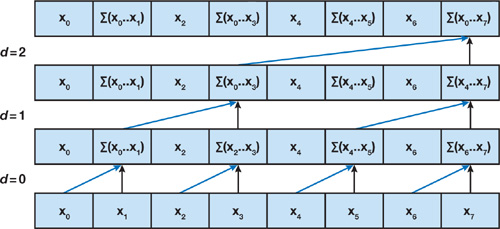
\includegraphics{parallelScanUpSweep.jpg}
		\caption{Up-Sweep -Phase des Work Efficient Parellel Scan; Quelle: \cite{Harris2007} }
		\label{fig:parScanUpSweep}
		\end{figure}
		
		\begin{figure}[!h]
		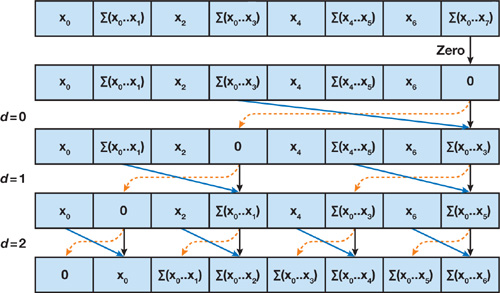
\includegraphics{parallelScanDownSweep.jpg}
		\caption{Down-Sweep -Phase des Work Efficient Parellel Scan; Quelle: \cite{Harris2007} }
		\label{fig:parScanDownSweep}
		\end{figure}
		
		Die vorgestellte Implementierung berücksichtigt und löst die sog. \emph{Bank Conflicts}, welche
		bei Nvidia-GPUs auftreten, wenn auf verschiedene Bereiche des Local Memory gleichzeitig 
		zugegriffen wird, und wenn das Intervall zwischen den Speicherzugriffen ein Vielfaches der
		Anzahl an Banks ist. Im Falle von Bank Conflicts müssen die Zugriffe sequentialisiert werden.
		Das Access Pattern auf den Local Memory wird mit steigender Tiefe
		des Sweeps aufgrund der größer werdenden Abstände zwischen den Array-Einträgen immer Bank Conflict-anfälliger,
		daher ist ihre Vermeidung bei diesem Algorithmus besonders wichtig.
		
		
		%-----------------------------------------------------------------------------		
		
		\subparagraph{Parallel Radix Sort und Stream Compaction}
		Auf den \emph{Work Efficient Parallel Prefix Sum} bauen der 
		\emph{Parallel Radix Sort} und die \emph{Stream Compaction} auf.\\
		Der Parallel Radix Sort wird in \cite{Grand2008} beschrieben.

		In der Fluid-Simulation wird ein Sortier-Verfahren benötigt, weil
		für Nähe im Speicher (wichtig für Coalesced Reads) und für die Nachbarschafts-Suche 
		über das Uniform Grid die Partikel anhand einer \emph{Z-Order-Curve} (siehe \cite{wiki:ZCurve}) sortiert werden 
		müssen.
		Die Z-Order-Curve gewährleistet eine gewisse räumliche Nähe zwischen den im Speicher benachbarten Zellen,
		was der Cache-Hit-Rate erhöht.
		
		Ein Array von Integer-Keys wird in mehreren Phasen nach ihren Key-Werten sortiert;
		In jeder Phase wird nach einem anderen Bit-Intervall in der Binär-Repräsentation der Keys
		sortiert. Da das Verfahren stabil ist, sich also die Reihenfolge zwischen Array-Elementen,
		deren Werte vom momentanen Sortier-Kriterium unabhängig sind, nicht ändert, ist dieser
		Mehr-Phasen-Ansatz ohne	weiteres möglich.
		Die Sortierung geschieht durch mehrstufige Scans von sog. \emph{Radix Counters}:
		Es existieren pro Sortier-Phase $2^{numBitsToSortPerPhase}$ Radix Counter Sets, einen pro
		Binär-Wert, den das momemtan betrachtete Binär-Intervall annehmen kann.
		Beispiel: Sortiert man in Intervallen @ 6 Bit, braucht man $2^6=64$ Radix Counter Sets.
		Ein Counter Set ist ein Array, welches so lang sein kann wie das zu sortierende Eingabe-
		Array; es können sich aber auch mehrere Key-Elemente eine Counter-Gruppe teilen,
		je nach verfügbarem Speicher und Wunsch, die Counter-Arrays wegen des nicht unerheblichem Scan-Aufwandes
		klein zu halten.\\
		Das Schema eines Passes (ohne GPU-Implementations-spezifische Anpassungen) ist folgendes:
		\begin{itemize}
			\item Man inkrementiert den Radix Counter eines Keys, der dem Binärwert des betrachteten
			Bit-Intervalls entspricht. Wenn sich mehrere Keys eine Counter-Gruppe teilen, muss diese
			Inkrementation wegen Write-Hazards entweder mit atomaren Operationen geschehen, oder 
			aber sequentialisiert werden.
			\item Die Radix Counter Sets werden dann, jedes für sich, gescannt. Das Ergebnis gibt den
			\emph{Radix-lokalen} Offset eines Keys mit dem entsprechenden Radix an, also die relative
			Position eines Keys im später sortierten Array innerhalb des jeweiligen Array- Intervalls, 
			der zum entsprechenden Radix gehört.
			\item Die totale Summe, wie viele Keys mit einem bestimmten Radix existieren, fällt
			durch den Scan der Radix Counter Sets automatisch ab. Der Scan dieser Summen
			gibt den \emph{Radix-globalen} Offset an, also die Array-Position, wo das erste
			Key-Element eines bestimmten Radix im sortierten Array zu stehen hat.
			\item Die Key-Elemente und ggfs. assoziierten Werte werden dann anhand dieser beiden Offsets, die
			zum Radix des Keys gehören, gescattert.
		\end{itemize}
		Eine GPU-Implementation muss die Scans der beiden Offsets noch weiter unterteilen, um
		dem Umstand gerecht zu werden, dass die GPU aus mehreren nicht explizit synchronisierbaren
		Compute Units mit beschränktem Speicher, Recheneinheiten und verwaltbaren Work Groups besteht.
		
		Meine Implementation verwendet im Gegensatz zu \cite{Grand2008} atomics, um die Radix Counters
		zu inkrementieren, welche sich von mehreren Keys geteilt. Außerdem lade ich die Keys nach einem
		Schema auf den Local Memory herunter, dass nur die ersten $n$ Work items daran beteiligt sind.
		Auf diese Weise ergeben sich weniger aktive Warps für diesen Vorgang.
		Ferner, weil mehr Work Items pro Work Group existieren als ein Compute Unit-lokales
		Radix Counter Set lang ist (aufgrund des beschränkten Local Memory), werden gleich mehere
		Radix Counter Sets von einer Work Group parallel gescannt.\\
		
		%---------------------------------------------------------------------
		
		Die \emph{Stream Compaction} funktioniert wesentlich einfacher als der Radix Sort:
		es wird anhand eines Kriteriums bestimmt, ob ein Array-Element im Ausgabe-Array enthalten sein soll oder nicht.
		Je nach dem wird in ein Array der gleichen Länge wie das Eingabe-Array eine Null oder eine Eins geschrieben.
		Dieses Array wird dann gescannt. Das Ergebnis des Scans gibt die neue Array-Position der
		Key-Elemente an, die im Ausgabe-Array enthalten sein sollen. Jene Keys werden gescattert, die anderen
		Keys nicht herausgeschrieben. Somit ergibt sich ein komprimiertes Array, welches nur bestimmte
		Keys des Eingabe-Arrays enthält.\\
		Die \emph{Stream Compaction} wird benötigt, um den Particle Count der Uniform Grid-Zellen
		in OpenCL Work Groups zu transformieren (siehe \cite{Goswami2010}):
		Leere Zellen werden heraus geschmissen, die vollen Zellen
		gegebenenfalls aufgespalten und komprimiert herausgeschrieben. Somit ergibt jede
		komprimierte Zelle einen Start-Punkt für eine SPH-Work Group: Die Work Group erfährt durch die Zelle
		den Start-Index der Partikel in den Radix-sortierten Partikel-Attribute-Arrays und die Anzahl an
		Partikeln, die sie abzuarbeiten hat. Jede weitere für die SPH-Kernels relevante Information
		lässt sich dann aus den Partikel-Attributen ermitteln.
		
		
		
		
	\paragraph{Ablauf}
		\label{sec:fluidSim:ablauf}
		
		Es gibt zwei OpenCL-Kernels, die anstelle der Standard-Kernels im allerersten Simulations-Schritt genutzt werden
		müssen: Zum einen ein Z-Index-Berechnungs-Kernel, der aus den 3D-Weltpositionen einen Index
		gemäß der erwähnten Z-Order-Curve berechnet (siehe Abb. \ref{fig:zOrderCurve}). 
		In allen weiteren Schritten kann diese Berechnung
		im selben Kernel geschehen, wo auch die Integration passiert.
		Zum anderen benötigt das verwendete \emph{Velocity Verlet}-Integrations-Schema 
		(s. \cite{Eberly2004}, S. 483 ff.) zwei Geschwindigkeits-Werte (predicted/corrected) und die Beschleunigung
		aus dem vorherigen Simulations-Schritt.
		Deshalb braucht es einen Kernel, der eine initiale Integration ohne alte Beschleunigung und mit nur einem
		Geschwindigkeits-Wert macht.
		
		\begin{figure}[h]
		\centering
		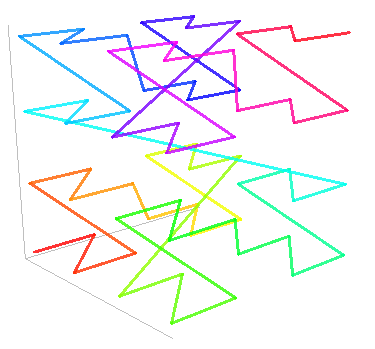
\includegraphics[width=0.33\textwidth]{ZOrderCurveWiki.png}
		\caption{3D-Z-Order-Curve; Quelle: \cite{wiki:ZCurve} }
		\label{fig:zOrderCurve}
		\end{figure}
		
		Ansonsten läuft ein Simulations-Schritt wie folgt ab:
		\begin{enumerate}
			\item Sortiere Z-Indices mit dem "`oldIndices"'-Buffer per \emph{Parallel Radix Sort}.
			\item Ordne die Partikel-Attribut-Buffers neu an mithilfe des "`oldIndices"'-Buffer.
			\item Aktualisiere das Uniform Grid anhand der sortierten Z-Indices.
			\item Komprimiere das Uniform Grid per \emph{Stream Compaction}.
			\item Lese die totale Summe Stream-Compaction-Scans aus; 
				dieser gibt die Anzahl an benötigten SPH-Work Groups an.
			\item Berechne die Dichte per SPH.
			\item Berechne Kraftdichten durch Druck und Viskosität per SPH, füge Gravitation, Benutzer-Einwirkungen und 
			Mesh-Kollisions-Kräfte hinzu, dann integriere mit Verlocity Verlet und berechne den neuen Z-Index.
		\end{enumerate}
		

	\paragraph{Optimierungen}
	\label{sec:hardwareOptimizations}
		
		\subparagraph{"`multi-parallel Scan"'}
			Wie erwähnt kann meine Implementation, falls nötig und sinnvoll, mehrere kleine Arrays pro 
			Work Group gleichzeitig scannen.
	
		\subparagraph{Cache}
			Der Benutzer kann per Config einstellen, ob eine implizit Cache-nutzende (in Hinblick auf die
			Fermi-Architektur) Implementation der SPH-Kernels genutzt werden soll, welche nicht 
			wie in \cite{Goswami2010} den Umweg geht,
			Nachbar-Partikel in den Local Memory herunter zu laden und anschließend zu synchronisieren.
		
		\subparagraph{Größe des Local Memory}
			Je nach verfügbarem Local Memory ändert sich die Mögliche Anzahl an verfügbaren
			Radix Counters pro Work group. Die anderen Parameter (z.B. Anzahl an Key Elements, die sich einen
			Counter teilen) werden für optimierte Performance entsprechend angepasst.
			
	
		\subparagraph{Bugs}
		\label{sec:oclBugs}
		Während der Implementierung sind mir einige Dinge aufgefallen, die ich auf Bugs im OpenCL-Treiber
		oder zumindest auf Beschränkungen der spezifischen OpenCL-Implementation zurück führe.
		Ich will nicht ausschließen, dass es sich vielleicht um eigene Programmierfehler handelt, jedoch habe ich
		viel herum probiert und meinen Code inspiziert, und mit bestimmten Code-Konstrukten, die eigentlich
		rein semantisch äquivalent sein müssten zu den Konstrukten, mit denen es Abstürze und/oder einen sonderbaren
		Simulationsverlauf gibt, funktioniert es dann.
		Teilweise ergaben sich mit einer Geforce GTX280 (Nvidia GPU der GT200-Architektur) 
		Bugs, die auf einer Geforce GT435M (Fermi-Architektur) nicht auftraten.
		Dies kann z.T. an Architektur-spezifischen Unterschieden in den Treibern liegen, am verwendeten
		CUDA-Toolkit oder an dem signifikanten Unterschied bei der Anzahl an Compute Units (30 vs 2), die die
		GTX 280 potentiell anfälliger für Synchronisationsprobleme machen könnte.
		
		\begin{enumerate}
		
			\item Absturz bei globalen Speicherzugriffen (Lesen wie Schreiben) innerhalb von Schleifen, 
			wo sich die Schleifen-Lauf-Variablen zwischen den einzelnen work items einer
			Work Group unterscheiden:
			\begin{lstlisting}[language=OpenCL]
for(uint simGroupRunner=0; simGroupRunner < numSimWorkGroupsOfThisCell; simGroupRunner++ )
{
	//numSimWorkGroupsOfThisCell is different between work items here!
	/*global mem acces --> crash!*/
			\end{lstlisting}
			
			Work-Around: Feste Schleifen-Länge, Schleifen-Abbruch per \lstinline|break|, wenn eigentliche
			Schleifenbedingung nicht mehr gilt:
			\begin{lstlisting}[language=OpenCL]
for(uint simGroupRunner=0; simGroupRunner <  NUM_MAX_ALLOWED_UNIGRID_CELL_SPLIT_FACTOR; simGroupRunner++ )
{
	if( simGroupRunner >= numSimWorkGroupsOfThisCell )
    { break; }
    /*global mem acces --> works!*/
			\end{lstlisting}
			
		\item Bei wiederholtem lesenden Zugriff auf die selbe Stelle im 
		globalen Speicher innerhalb eines Schleifenrumpfes (selbst wenn Werte in eine 
		\lstinline|__private| -Variable zwischengespeichert und diese im Anschluss durchgehend genutzt werden),
		verhält sich die Simulation so, als ob bestimmte (andere als die erste)
		Operationen gar nicht ausgeführt worden wären. Es bestehen keinerlei Datenabhängikeiten zwischen
		den Operationen dieses Schleifenrumpfes.
		Dieses Problem tritt nur mit der GTX280 auf, nicht mit den Fermi-Karten.
		\begin{lstlisting}[language=OpenCL]
for(  uint interactingLocalIndex=0; 
           interactingLocalIndex < numNeighbourParticlesToInteractWith;
           interactingLocalIndex++ )
{  
	/*calc pressure force reading density twice and position once 
	from global mem resp. from just-refreshed private variable*/ 
	
	//barrier(CLK_LOCAL_MEM_FENCE); //<-- on GTX 280, this barrier must be commented in; 
	//it doesnt matter if its GLOBAL oder LOCAL memory fence, this is weird, as there is no local memory accces at all
	//with this kernel setup; 
	//On GT 435M, it works fine without this barrier...
	
	/*	calc viscosity force reading density once and density once from global mem 
		resp. from same private variable as for pressure calc
		<-- simulation acts like if there were no viscosity calculation at all without barrier!*/
}
		\end{lstlisting}
		
		\item 
		\label{enum:oclSyncBug}		
		Mit steigener Anzahl an Compute-Units und Partikeln wird die Simulation unter folgenden Umständen immer instabiler:
		Verteile ich den Scan, der für die Stream Compaction nötig ist, auf mehre Compute Units statt nur einer,
		so dass im Compaction Kernel pro Work Group noch ein kleiner finaler Scan gemacht werden muss,
		der die Teil-Summen der verschiedenen Scan-Work Groups aufsummiert, poppen Partikel
		in Zellen oder ganzen Zell-Blöcken weg, häufig friert die Anwendung ein.
		Mit nur einer Compute Unit, die diesen Kernel abarbeitet, also nur einer Work Group, ist die Simulation stabil.
		
		Von den bisher erwähnten Bugs halte ich es hier für am wahrscheinlichsten, dass es sich um einen Programmierfehler 
		meinerseits handelt, auch wenn ich bereits viel über diesen Kernel gegrübelt habe.
		
		Letztendlich ist der Kernel, der den Scan zu Stream Compaction macht, recht klein im Vergleich zu den
		Radix-Sort- und SPH-Kernels; Daher ist es für die Performance nicht so tragisch, wenn hier nur eine Work 
		Group aktiv ist; ärgerlich ist es trotzdem.
		\end{enumerate}

\clearpage
